\documentclass{article}
\usepackage{parskip}
\usepackage{amsmath}
\usepackage{graphicx}
\graphicspath{ {./} }
\usepackage{tikz}
\usetikzlibrary{shapes.geometric, arrows, plotmarks}
\tikzstyle{startstop} = [rectangle, rounded corners, minimum width=3cm, minimum height=1cm, text centered, draw=black]
\tikzstyle{process} = [rectangle, minimum width=3cm, minimum height=1cm, text centered, draw=black]
\tikzstyle{decision} = [diamond, aspect=2, minimum width=3cm, minimum height=1cm, text centered, draw=black]
\tikzstyle{arrow} = [thick,->,>=stealth]
\usepackage{float}
\usepackage{listings}
\usepackage{pgfplots}

\setlength{\belowcaptionskip}{10pt}

\title{Project 2: Parallel Fluid Dynamics Simulation}
\author{John Bradley}
\date{\today}

\begin{document}
  \maketitle

  \section{Introduction}

  This report aims to document the implementation and analysis of a program
  that utilizes OpenMP to implement a computational fluid dynamics model
  suitable for modeling behavior of turbulent flows. This report will cover the
  methods and techniques utilized for implementing the fluid dynamics model
  using OpenMP, analyze and estimate the expected performance of the 
  implementation, present the results from experimentation, compare and contrast 
  the expected performance to the observed results, and conclude with insights 
  and possible changes that could be made to the implementation
  
  \section{Methods and Techniques}

  Many of the functions in the code provided deal with sequential
  sections of memory, and allowing a single thread to access these sequential
  memory areas would be beneficial, as it would prevent cache contention
  between threads. Additionally, there are many nested loops, and the Ptolemy 
  system does not have \verb|OMP_NESTED| set by default, thus the use of nested
  \verb|#pragma omp for| declarations should be avoided, as enabling nested
  parallel sections may not be beneficial. Careful partitioning of parallel 
  sections will be needed.

  For example, in the \verb|setInitialCOnditions| function, the inner-most
  nested loop contains:
  
  \begin{center}
    \begin{lstlisting}[language=C, linewidth=0.9\textwidth, breaklines=true]
for(int k=0; k<nk; ++k) {
  int indx = offset + k;
  float dz = (1./nk)*L;
  float z = 0.5*dz+k*dz - 0.5*L;

  u[indx] = 1.*coef*sin(x/l)*cos(y/l)*cos(z/l);
  v[indx] = -1.*coef*cos(x/l)*sin(y/l)*cos(z/l);
  p[indx] = (1./16.)*coef*coef*(cos(2.*x/l)+cos(2.*y/l))*(cos(2.*z/l)+2.);
  w[indx] = 0;
}
    \end{lstlisting}
  \end{center}

  For each iteration of the loop, \verb|indx| is the sum of \verb|offset|,
  defined in the outer loop, and the value of \verb|k|, which is incremented
  each iteration of the loop. If the loop was parallelized, each thread may
  access non-sequential sections of the \verb|u|, \verb|v|, \verb|p|, and
  \verb|w| arrays. If we, instead, parallelize the loop that contains the
  "\verb|k|" loop, then we can exploit this memory access pattern. This effect
  is more pronounced the further out this parallelization is declared.
  Furthermore, this prevents threads from trying to access memory locations
  that may be in the same cache line. 
  
  This pattern of access is present across many of the functions in the 
  program, and can be exploited in the same way. However, this na\"{i}ve 
  approach isn't applicable to all situations. For example, in 
  \verb|computeResidual|, the residual flux vectors (e.g. \verb|presid|, 
  \verb|uresid|, \verb|vresid|, and \verb|wresid|) are calculated using loops
  that may have overlapping read/write access.

  Creating a critical, or locked section, can ensure that more than one thread 
  does not update the variables at the same time, thus avoiding a race 
  condition. However, this will likely result in a performance impact as the 
  entire block is prevented from being entered by another loop. In fact, early 
  testing during development of the code showed that this does create a 
  significant performance impact.

  Looking closer at the \verb|offset| value and the two indexes for each
  component of the vector, the index of each vector's array is dependent on
  \verb|k| and the skip direction (\verb|i * iskip|, \verb|j * jskip|, 
  \verb|k * kskip|). This is true for the three loops calculating the vectors
  in each direction. Furthermore, the section of each loop where the vectors
  are accessed includes one of the three skip directions.

  \begin{center}
    \begin{lstlisting}[language=C, linewidth=0.9\textwidth, breaklines=true]
    \end{lstlisting}
  \end{center}

  \begin{center}
    \begin{lstlisting}[language=C, linewidth=0.9\textwidth, breaklines=true]

#pragma omp parallel
{
  #pragma omp for
  for(int j=0; j<nj; ++j) {
    const float vcoef = nu/dx;
    const float area = dy*dz;
    for(int i=0; i<ni+1; ++i) {
      int offset = kstart+i*iskip+j*jskip;
      for(int k=0; k<nk; ++k) {
        const int indx = k+offset;
    
...

      }
    }
  }
}

    \end{lstlisting}
  \end{center}

  Simply swapping the \verb|i| and \verb|j| loops in the first vector
  calculation kept the integrity of the data while eliminating the need for
  variable locks. The second and third calculation in \verb|computeResidual| do
  not need to have the loops reordered as they are not parallelizing two index
  locations next to each other.

  Finally, some functions, such as \verb|computeStableTimestep|, requires that
  a minimum be reduced from the parallelization portion. In C++, if this was a
  mathematical operation, such as summation or subtraction (such as in
  \verb|integrateKineticEnergy|), this would be a trivial task using a built-in
  reduction clause. However, it is not. To prevent a race condition, a minimum
  local to the thread must be calculated, and once that is done, a critical
  section is added so that only one thread does a global (or team) comparison
  to set the final minimum value.

  \begin{center}
    \begin{lstlisting}[language=C, linewidth=0.9\textwidth, breaklines=true]

float minDt = 1e30;
#pragma omp parallel
{
  float local_minDt = 1e30;
  #pragma omp for nowait
  for(int i=0; i<ni; ++i) {
    for(int j=0; j<nj; ++j) {
      int offset = kstart+i*iskip+j*jskip;
      for(int k=0; k<nk; ++k) {
        const int indx = k+offset;

        // inviscid timestep
        const float maxu2 = max(u[indx]*u[indx],max(v[indx]*v[indx],w[indx]*w[indx]));
        const float af = sqrt(maxu2+eta);
        const float maxev = sqrt(maxu2)+af;
        const float sum = maxev*(1./dx+1./dy+1./dz);
        local_minDt=min(local_minDt,cfl/sum);

        // viscous stable timestep
        const float dist = min(dx,min(dy,dz));
        local_minDt=min<float>(local_minDt,0.2*cfl*dist*dist/nu);
      }
    }
  }

  #pragma omp critical
  {
    minDT=min(minDT,local_minDt);
  }
}
    
    \end{lstlisting}
  \end{center}

  The \verb|nowait| clause was used so that the threads do not wait for other
  threads to reach the critical section before performing it.

  Further parallelization could be done, with each parallelized function being
  further parallelized using MPI, however this is outside of the scope of the
  undergraduate assignment.

  \section{Analysis}

  Very little of the code is spent in serial execution, as all of the functions
  were able to be parallelized to a great extent. A generious extimation of
  approximately 90\% of the execution time being parallelized gives us the
  serial fraction of:

  \[ f = \frac{W_S}{W_S + \sum W_K} = \frac{0.1}{1} = 0.1 \]

  based on the assumption that \( t_1 = 1 \). The upper bound of the speedup 
  is:

  \[ S_{upper} = \frac{1}{f} = \frac{1}{0.1} = 10 \]

  The upper bound can be compared to the estimated speedup for the number of
  procesors that will be used using the following equations:

  \[ t_p = \left[ f + \frac{\left( 1 - f \right)}{p} \right] \times t_1 \]

  \[ S = \frac{t_1}{t_p} \]

  \begin{table}[H]
    \centering

    \begin{tabular}{|c|c|}
      \hline
      Proc & Speedup \\
      \hline
      1  & 1                  \\
      2  & 1.$\overline{81}$  \\
      4  & 3.077              \\
      8  & 4.706              \\
      16 & 6.4                \\
      32 & 7.805              \\
      64 & 8.767              \\
      \hline
    \end{tabular}
    \caption{Estimated Speedup}
    \label{tab:estspeeduptab}
  \end{table}

  \begin{figure}[H]
    \centering

    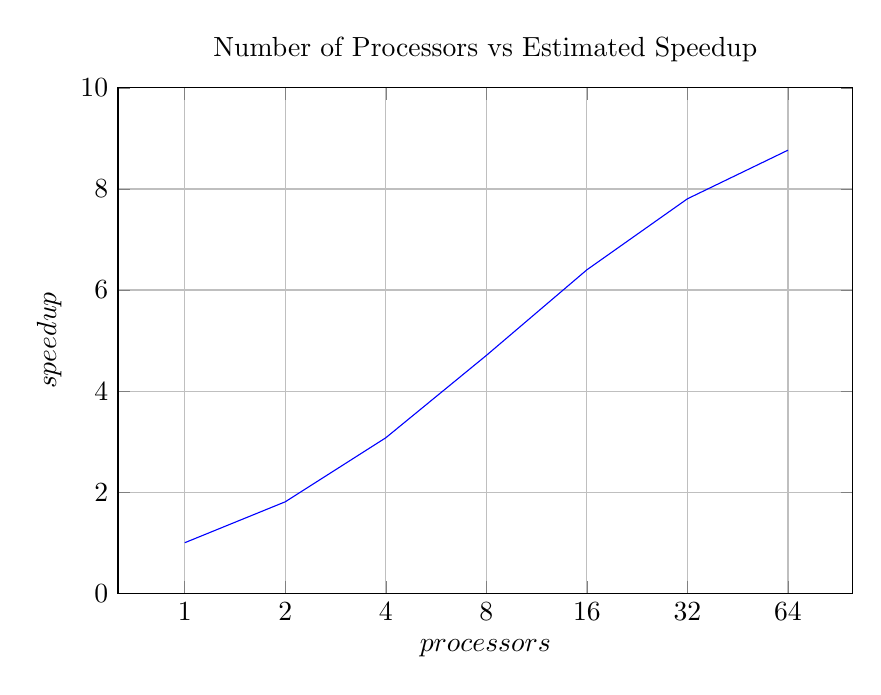
\begin{tikzpicture}
      \begin{semilogxaxis}[
        width=0.9\textwidth,
        height=8cm,
        xlabel={$processors$},
        ylabel={$speedup$},
        grid=both,
        ymin=0,
        ymax=10,
        xmax=100,
        xtick={1,2,4,8,16,32,64},
        xticklabels={1,2,4,8,16,32,64},
        title={Number of Processors vs Estimated Speedup}
      ]

      \addplot[blue,mark=none] coordinates {
        (1,1)
        (2,1.81)
        (4,3.077)
        (8,4.706)
        (16,6.4)
        (32,7.805)
        (64,8.767)
      };
      \end{semilogxaxis}
    \end{tikzpicture}
    \caption{Estimated Speedup}
    \label{fig:estspeedupfig}
  \end{figure}

  The estimated speedups are listed in Table~\ref{tab:estspeeduptab} and plotted
  in Figure~\ref{fig:estspeedupfig}.

  \section{Results}

 

  \section{Synthesis}

 

  \section{Conclusion}



\end{document}

